\label{sec:proj}

The computation proposed here will use the same ensembles of the previous stage of the project
i.e. Wilson-clover twisted
mass fermions~\cite{Alexandrou:2018egz}. The up/down quarks will be treated
in a fully unitary setting. To avoid flavor mixing lattice artifacts
in the unitary strange/charm sector of this regularization, we use a
mixed action approach for strange and charm quarks: so-called
Osterwalder-Seiler type~\cite{Frezzotti:2004wz} strange and charm quark doublets
$(s^+ , s^-)^T$ and $(c^+ , c^- )^T$ are added with bare
twisted strange and charm quark mass $\pm \mu_s$ and $\pm \mu_c$
tuned to reproduce the physical mass of the $\phi$ and $J/\Psi$
mesons, respectively, as described in Appendix C of
Ref.\cite{ExtendedTwistedMass:2022jpw}. For more details, we refer to
this reference.


The core of our project is the calculation of inclusive semileptonic
decays of the $B$ and $B_s$ mesons, for which we need to determine the
bare $b$-quark mass first.
For the application of what we call the
ratio-method~\cite{ETM:2009sed}, we will generate data at six
different values of the heavy quark mass in the range from 
1 to 3.5 times the charm quark mass. 
The data produced for these six heavy quark mass values can be used at
the same time for the  determination of the $B$ and $B_s$ meson masses
and the total inclusive decay rate for the process $B_{(s)} \to
X\ell\bar\nu$. 



%%%%%%%%%%%%%%%%%%%%%%%%%%%%%%%%%%%%%%%%%%%%%%%%%%%%%%%%%%%%%%%%%%%%%%%%%%%%%%%%%%
%%%%%%%%%%%%%%%%%%%%%%%%%%%%%%%%%%%%%%%%%%%%%%%%%%%%%%%%%%%%%%%%%%%%%%%%%%%%%%%%%%
\subsection{Sub-project 1: total inclusive decay rate $B_s \to X\ell\bar\nu$}

By using the optical theorem, the semileptonic decay of a $B$ and $B_s$
% mesons to charmed final states $X_c$ 
to a hadron $X$ with a pair of massless leptons $B_{(s)} \to X\ell\bar\nu$ can be written as
\begin{equation}
  \Gamma = G^2_F\left\{ |V_{bu} |^2 \Gamma_{bu} + |V_{bc} |^2 \Gamma_{bc} + |V_{su} |^2 \Gamma_{su}
  \right\}\,,
  % \Gamma_c = G^2_F |V_{bc} |^2 \Gamma_{bc}\,.
\end{equation}
where the different contributions to the right side correspond at the quark level
to the weak transitions $b \to u$, $b \to c$ and $s \to u$ respectively.
Each contribution can be written as
% This decay may occur with the quark-level decay process $b \to c\ell \bar\nu$, it's important to notice that in the case of the $B$ and $B_s$ meson this channel is known experimentally while 
% in the case of the $D_s$ meson only the sum over all weak transition is known. The decay rate divided by the square of the  Fermi constant $G_F$ and the CKM angle $V_{bc}$ can be written as
\begin{equation}\label{eq:Gamma_fg}
  \Gamma_{fg}=\int \frac{d^3p_\nu}{(2\pi)^32E_\nu}\frac{d^3p_\ell}{(2\pi)^32E_\ell}
  L_{\mu\nu}(p_\ell, p_\nu) H^{\mu\nu}_{fg}(p,p-p_\ell-p_\nu)\,,
\end{equation}
where the leptonic tensor is given by
\begin{equation}
  L_{\mu\nu}(p_\ell, p_\nu) =4\left\{p_\ell^\mu p_\nu^\nu +p_\ell^\nu
  p_\nu^\mu - g^{\mu\nu} p_\ell\cdot p_\nu+
  i\epsilon_{\mu\nu\alpha\beta} p_\ell^\alpha p_\nu^\beta\right\}\,,
\end{equation}
while the hadronic tensor reads
\begin{equation}
  H^{\mu\nu}_{fg}(p,p_X)=\frac{1}{2m_{B_{(s)}}}\langle B_{(s)}| J^\mu_{fg}(0)(2\pi)^4
  \delta^4(\mathbb{P}-p_x) J^{\nu\dagger}_{gf} (0)| B_{(s)}\rangle\,.
\end{equation}
$\mathbb{P}$ is the QCD four momentum operator and $J_{fg}$ are the
relevant Minkowski weak currents $J_{fd}^\mu(x)=i\bar
  f(x)\gamma^\mu(1-\gamma_5)g(x)$.
The contribution $\Gamma_{su}$ is zero in the decay of the $B$ for momentum conservation while  in the decay of the $B_{s}$
is suppressed by the integration over
the phase space of \eqref{eq:Gamma_fg}, moreover, this  channel is only inclusive through $B_s-> B\ell\bar\nu$.
% The $bu$ channel for the $B$ meson involves disconnected contribution
The calculation of $\Gamma_{bu}$  requires computing disconnected diagrams which is computationally more challenging than the connected part.
On the other hand the contribution coming from disconnected diagrams is expected to be small due to OZI-suppression rule.
In this project we will focus only on the computation of $\Gamma_{bc}$ and the connected part of $\Gamma_{bu}$
leaving the computation of the disconnected diagram in a separate project.
It is important to notice that the decays $B_{(s)} \to X_c\ell\bar\nu$ corresponding to decays into charmed final states $X_c$ are known from the experimental side and thus can be compared directly with our calculations.

% In this channel there are not disconnected diagrams.
% On the contrary of the decay of the $D_s$ meson here there are not disconnected
% diagrams.
% The contribution $\Gamma_{su}$ is suppressed by the integration over
% the phase space of \eqref{eq:Gamma_fg} thus it is expected to not contribute to the total
% decay rate. Moreover, the decay in the $su$ channel is only inclusive through $B_s-> B\ell\bar\nu$.
% In this project we will focus only on the $bu$ and $bc$ channels while we will verify
% that the $su$ contribution is small in separate budget available on other machines.
From now on we will drop the indices $fg$
and the procedure we are describing will be equivalent for the $bu$ and $bc$ contributions,
moreover
in the rest frame of the $B_{(s)}$ meson we have $p=(M_{B_{(s)}},\bm{0})$ thus we simplify the notation of
$H^{\mu\nu}(p_X)\equiv H^{\mu\nu}_{fg}(p,p_X)$.
The hadronic tensor $H_{\mu\nu}$ is
the spectral density of the quantity
\begin{equation}
  M_{\mu\nu}(t,{\bf q})= \int_0^{\infty}d \omega H_{\mu\nu} (\omega,{\bf q}) e^{-\omega t}\,,\quad \text{with}\quad p_X=(\omega,\bm{q})\,.
\end{equation}
$H_{\mu\nu}$ can be reconstructed from $M_{\mu\nu}$ using the method presented in
Ref.~\cite{Hansen:2019idp}. $M_{\mu\nu}$ can be directly computed from the
ratio of Euclidean lattice correlators
\begin{gather}
  M_{\mu\nu}(t_2-t_1,{\bf q})=\frac{C_{\mu\nu}(t_{snk},t_2,t_1,t_{src};q)}{e^{-(t_{snk}-t_2)}  C(t_1-t_{src}) }\label{eq:ratio_4pt_2pt}\\
  \label{eq:4pt}
  C_{\mu\nu}(t_{snk},t_2,t_1,t_{src};q)=\int d^3x e^{i{\bf q}\cdot {\bf x}}
  \langle B_{(s)}({\bf 0}, t_{snk}) J^{\dagger}_\mu({\bf x},t_2)  J_\nu(0,t_1)
  B_{(s)}^\dagger({\bf 0}, t_{src})\rangle\,,\\
  \label{eq:2pt}
  C(t_{snk}-t_{src}) =  \langle B_{(s)}({\bf 0}, t_{snk})
  B_{(s)}^\dagger({\bf 0}, t_{src})\rangle\,.
\end{gather}
In general, the inverse problem represented by the extraction of
hadronic spectral densities from Euclidean correlators is notoriously
ill-posed. Recently, a method to cope with these problems has been
proposed in Ref.~\cite{Hansen:2019idp}. It consists of treating the
integrals mentioned above with some $C_\infty$ kernel $K_\sigma$
\begin{equation}
  H^\sigma_{\mu\nu}(\omega^*, {\bf q})= \int d \omega K_\sigma( \omega^*,\omega ) H_{\mu\nu}(\omega, {\bf q})\,,
\end{equation}
making the inverse problem well posed and $H^\sigma_{\mu\nu}$ computable.
In our case the phase space integration in \eqref{eq:Gamma_fg}
provides a sharp smearing kernel function $\theta$. Following
Refs.~\cite{Gambino:2020crt, Gambino:2022dvu}, the phase space integral over
\eqref{eq:Gamma_fg} can be written as
\begin{gather}
  \frac{48 \pi^4}{m_{B_{(s)}}^5}\frac{d\Gamma}{d \bm{ \omega^2} }
  =\sum_{l=0}^2 |\bm{\omega}|^{3-l}\int_0^{\infty}d \omega_0 \Theta^l(\omega_0^{max}-\omega_0) Z^l\,,\quad\quad {\omega}_0^{max}=1-|\bm{\omega}|\,,\quad\Theta^l(x)=x^l\theta(x)\\
  Z^2=Y_3-2Y_1\,,\quad Z^1=2(Y_3-2Y_1-Y_4)\,,\quad Z^0=Y_2+Y_3-2Y_4\,.
\end{gather}
Moreover, the $Y_i$ can be directly computed from the Euclidean
hadronic tensor $H^{\mu\nu}$ as follows
\begin{align}
                                                     & Y^1=-m_{B_{(s)}}\sum_{ij}\hat{n}^i\hat{n}^j H^{ij}(p,q)\,,          &  & Y^2=-m_{B_{(s)}}H^{00}(p,q)\,, \\
                                                     & Y^3=m_{B_{(s)}}\sum_{ij}\hat{\omega}^i\hat{\omega}^j H^{ij}(p,q)\,, &  &
  Y^4=-im_{B_{(s)}}\sum_{i}\hat{\omega}^i H^{0i}(p,q)\,, &
\end{align}
with $\hat{n}$ a unit vector orthogonal to $\bm\omega$.
Thus, the phase space integral provides us a $\theta$-function smearing
kernel. However, the $\theta$-function is not smooth, which is why we
will use a $C_\infty$ kernel that
after taking the infinite volume limit, the
$\theta$-function is recovered as $\sigma\to0$, i.e. $\lim_{\sigma\to 0} K_\sigma^l(x^*,x)=\Theta^l(x^*-x)$.
%such that the step-function is recovered in the limit $\sigma\to0$, i.e.
%$\lim_{\sigma\to 0} \theta_\sigma(x)=\theta(x)$.
Therefore,
\begin{gather}
  \frac{48 \pi^4}{m_{B_{(s)}}^5}\frac{d\Gamma}{d \bm{ \omega^2} }
  =\lim_{\sigma\to 0}\sum_{l=0}^2 |\bm{\omega}|^{3-l}\int_0^{\infty}d \omega_0 K_\sigma^l(\omega_0^{max},\omega_0) Z^l\,.
\end{gather}
The spectral reconstruction can be performed at the analysis stage. Thus,
the main cost of this calculation is the production of the
four-point function \eqref{eq:4pt}.
% In the case of the $b\to u$ weak
% transition the corresponding required Wick contractions are shown in
% Fig.~\ref{fig:4pt}.

The renormalization constants necessary to renormalise the ratio of
correlators \eqref{eq:ratio_4pt_2pt} $Z_A$ and $Z_V$ are already
computed in previous work of ETMC~\cite{ExtendedTwistedMass:2024myu}.

\begin{figure}
  \centering
  \begin{tikzpicture}
    \begin{feynman}[scale=1.5]
      \vertex[anchor=east,blob, fill=black!0!] (a) at (0,0) {\(B_{(s)}^\dagger\)};
      \vertex[anchor=east,blob, fill=black!0!]  (J1) at (1,0.8) {\(J_W\)};
      \vertex[anchor=east,blob, fill=black!0!] (J2) at (2.4,0.8) {\(J_W\)};
      \vertex[anchor=west,blob, fill=black!0!] (b) at (3,0) {\(B_{(s)}\)};
      \vertex (s1) at (3.4,-0.4) ;
      \vertex (s2) at (3.4, 0.4) ;
      \vertex (s3) at (2.6, 0.7) ;
      \vertex (s4) at (1.8, 1) ;

      \diagram*{
      %				(a) --[fermion,  half right,looseness=0.5,edge label=$s$] (b);
      (b) --[fermion, black, out=220, in=320,edge label=$u(s)$,swap] (a);

      (a) --[fermion, blue, edge label=$b$] (J1) ;
      (J1) --[fermion, sand, edge label=$c$, reversed momentum'=$\bf{q}$] (J2);
      (J2) --[fermion, blue ,edge label=$b$] (b);
      (s1) --[->, half right, edge label=sequential,swap] (s2);
      (s3) --[->, half right, edge label=sequential,swap] (s4);
      };
    \end{feynman}
    \begin{feynman}[scale=1.5]
      \vertex[anchor=east,blob, fill=black!0!] (a) at (6.5,0) {\(B_{(s)}^\dagger\)};
      \vertex[anchor=west,blob, fill=black!0!] (b) at (9.5,0) {\(B_{(s)}\)};

      \diagram*{
      %				(a) --[fermion,  half right,looseness=0.5,edge label=$s$] (b);
      (b) --[fermion, black, out=220, in=320,edge label=$u(s)$,swap] (a);
      (a) --[fermion, blue, out=40, in=140,edge label=$b$,swap] (b);
      % (a) --[fermion, green!40!black, out=40, in=140,edge label=$b$,swap] (b);
      };
    \end{feynman}
  \end{tikzpicture}
  \caption{On the left: Wick contractions required for the calculation of the correlator \eqref{eq:4pt} for the contribution $cd$. For the contribution $cs$ the $d$-quark propagator must be replaced with and $s$-quark propagator. On the right: Wick contractions required for the calculation of the correlator \eqref{eq:2pt} .}
  \label{fig:4pt}
\end{figure}

A similar analysis was done in the first stage of the project and the result
are shown in Fig.~\ref{fig:dGammadq_Ds} already extrapolated to the continuum and
to $\sigma\to0$.
The extra difficulties will come from the fact we can not simulate directly at the
physical $b$-quark, but the decay rate will be computed
using a set of heavy quark mass as described in the sub-project 2 of section~\ref{sec:mb}
and then extrapolated to the physical $b$ mass.

% As mentioned already, we have performed a first exploratory
% investigation of the differential decay rate on ensemble cB211.072.64
% in order to understand the feasibility of the proposed calculation. We
% used 300 gauge configurations with three stochastic sources each
% (see below for how stochastic sources are used here)
% and we compute only the $cd$ contribution. The
% resulting differential decay rate is shown in Fig.~\ref{fig:dGammadq_Ds}
% for four values of the square momentum of the final hadronic state. Apart from the statistical
% accuracy, which appears satisfactory, we also wanted to understand how
% to choose the time-separations appropriately. For one of the values of
% the momenta we have performed the calculation for different choices
% for the times $t_{snk}$, $t_2$ and the minimal value of $t_1$ included
% in the spectral reconstruction. However, within errors, all three
% choices give compatible results.

% For the calculation proposed here we plan to stick to the most
% conservative choice, namely $t_{snk}=56$, $t_2=40$ and $t_1=16$,
% corresponding to the blue circles in Fig.~\ref{fig:dGammadq_Ds}.
% For the ensembles at the other lattice spacings and volumes we plan to keep the
% time separations constants in physical units.


\begin{figure}
  \centering
  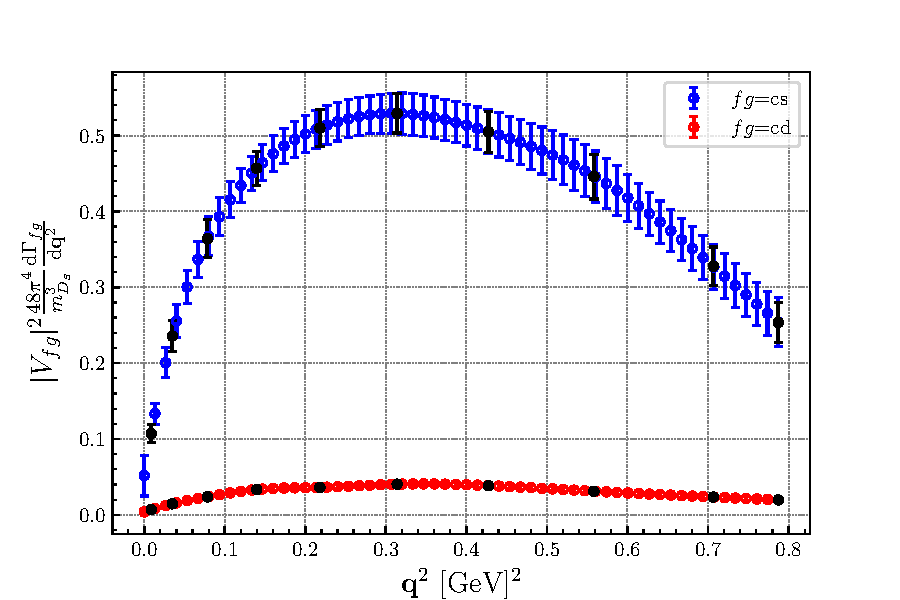
\includegraphics[scale=0.8]{plots/final_DgammaDq2.pdf}
  \caption{Preliminary values of the differential decay rate of
  $D_s\to X\ell\bar\nu$.
  the contribution form the $cd$ channel (in red) is observed to be smaller than
  the contribution form the $cd$ channel and (in blue) mainly due to $V_{cs}>V_{cd}$ }
  \label{fig:dGammadq_Ds}
\end{figure}

% \subsection{Sub-project 2: decay constant $f_D$ and $f_{D_s}$}

% From the two-point function \eqref{eq:2pt} we can extract the decay
% constant of the corresponding pseudo-scalar (PS) meson as 
% \begin{equation}
%   f_\mathrm{PS}=(\mu_f+\mu_{f'})\frac{\langle 0| P_{ff'}|
%     \mathrm{PS}\rangle}{M_\mathrm{PS}^{ff'}\sinh(M_\mathrm{PS}^{ff'})}\, 
% \end{equation}
% where the matrix element is extracted from the correlation function
% \eqref{eq:2pt} at large time separations. The PS-meson is made out of
% valence quark flavours with bare masses $\mu_f$ and $\mu_{f'}$ , and
% its mass is denoted by $M_\mathrm{PS}^{ff'}$. We plan to compute the
% decay constant for the $D_s$ and $D$ meson, thus $f=c$ and $f'=s,d$. 


\subsection{Sub-project 2: Bottom quark mass $m_b$}
\label{sec:mb}

In this sub-project we describe the determination of the $b$-quark
mass. We can extract the mass of the $B$ and $B_s$ pseudo-scalar mesons ($M_{B}$ and $M_{B_s}$)
from the right diagram of Figure~\ref{fig:4pt} representing the two-point function
\begin{equation}
  \langle B_{(s)}(\bm{0},t) B_{(s)}^\dagger({\bf 0},0)\rangle\xrightarrow{t>>a, (T-t)>>a}
  \frac{1}{2M_{B_{(s)}}}|\langle 0 | B_{(s)} | B_{(s)}\rangle|^2\left(e^{-M_{B_{(s)}} t}+e^{-M_{B_{(s)}}(T-t)}\right)
  \,
  \label{eq:Mb}
\end{equation}
with the operators $B({\bf 0},t)=\frac{1}{L^3}\sum_{\bf x}\bar b\gamma_5 u({\bf x},t)$
and $B_s({\bf 0},t)=\frac{1}{L^3}\sum_{\bf x}\bar b\gamma_5 s({\bf
  x},t)$.
In quantities involving the (valence) $b$-quark, we expect lattice
artifacts of the order $(am_b)^2$, which can be significant even with
the lattice spacing values employed in this project. Therefore, it is
advisable not to work directly at the $b$-quark mass, but to apply the
ratio method: The $b$-quark mass is obtained as an interpolation
between quark masses in the charm region and the static limit.
Thus, we compute Eq.~(\ref{eq:Mb}) replacing the $b$ quark with six heavy quarks $h$
in the range of $m_h\in [m_c,3.5m_c]$
and for each we compute the ratio
\begin{equation}
  Q_m = \frac{M_{hs}}{M_{h\ell}^\gamma M_{cs}^{(1-\gamma)}}\,,
  \label{eq:ratio_Q}
\end{equation}
where $M_{hs}$ and $M_{hl}$ are the heavy-strange and heavy-light
pseudoscalar masses, respectively, while we denote by $M_{cs}$
the mass of the pseudoscalar meson made out of a charm
and a strange quark. The parameter $\gamma$ is a free parameter in the range $[0, 1)$.
The asymptotic behavior of $Q_m$ can be computed using HQET reading
\begin{equation}
  \lim_{ m^{pole}_h\to \infty}
  \frac{M_{hs}}{( m^{pole}_h)^{(1-\gamma)} M_{h\ell}^\gamma}=\mbox{const.}\,,
  \label{eq:yHQFTlim}
\end{equation}
where $ m^{pole}_h$ is the pole mass of the heavy quark.
We then consider a sequence of heavy quark masses such that any two
successive masses have a common and fixed ratio i.e.
$ m_h^{(n)}=\lambda m_h^{(n-1)}, n=2,3,...$ and we construct the
follosing ratios at given lattice spacing $a$
\begin{equation}
  \begin{split}
    y_Q( m^{(n)}_h,a)&=\frac{Q_m( m_h^{(n)},a)}{Q_m( m_h^{(n-1)},a)}\cdot
    \left(\frac{ m_{h}^{(n)} \rho( m_{h}^{(n)})}{ m_{h}^{(n-1)}\rho( m_{h}^{(n-1)})}\right)^{(\gamma-1)}\\
    &=\lambda^{(\gamma-1)}\frac{Q_m( m_h^{(n)},a)}{Q_m( m_h^{(n-1)},a)}\cdot
    \left(\frac{ \rho( m_{h}^{(n)})}{\rho(
      m_{h}^{(n-1)})}\right)^{(\gamma-1)}\\\,,
  \end{split}
\end{equation}
where we have used the relation  $ m^{pole}_h= m_{h}^{} \rho( m_{h}^{})$
between the $\overline{\mbox{MS}}$ renormalised mass and the pole
mass, which is known perturbatively up to N$^3$LO~\cite{Chetyrkin:1999pq}.
For each pair of heavy quark masses, we carry out a continuum
extrapolation seperately
\footnote{We do not need a chiral extrapolation since we are already at physical point.}
obtaining $y_Q( m^{(n)}_h)=y_Q( m^{(n)}_h,a=0)$.
In the continuum limit, the ratios $y_Q( m^{(n)}_h)$ can be described
in terms of the heavy mass $m_h$ as~\cite{ETM:2011zey}
\begin{equation}
  y_Q( m^{(n)}_h) = 1 + \frac{\eta_1}{ m_h}+ \frac{\eta_2}{ m_h^2}\,,
  \label{eq:fity}
\end{equation}
where $\eta_{1,2}$ are free parameters and the limit in
Eq.~(\ref{eq:yHQFTlim}) has already been taken into account.
Finally, the $b$-quark mass can be computed with
\begin{equation}
  y_Q( m^{(2)}_h)y_Q( m^{(3)}_h)...y_Q( m^{(K+1)}_h)\frac{Q_m( m_h^{(1)},a)}{\lambda^{K(\gamma-1)}}
  \left(\frac{ \rho( m_{h}^{(K+1)})}{\rho( m_{h}^{(1)})}\right)^{(1-\gamma)}=Q_m( m_h^{(K+1)},a)
  \,,
\end{equation}
where the ratios $y_Q$ on the left-hand-side are evaluated using the
fit function Eq.~(\ref{eq:fity}) and the parameters $\lambda$, $K$ and
$ m_h^1$ chosen such that $Q_m( m_h^{(K+1)},a)$ matches 
the experimental value of the ratio $M_{B_s}/(M_{B}^\gamma M_{D_s}^{(1-\gamma)})$.


\endinput
